\documentclass[%singlesided,
               doublesided,
               paper=a4,
               fontsize=10pt
              ]{my-resume}

%% PUBLICATION LIST

\usepackage[backend=biber,style=apa,sorting=ydnt,uniquename=false,isbn=false,maxbibnames=99,url=false,giveninits=true,eprint=false]{biblatex}
\AtEveryBibitem{\clearfield{note}}
\addbibresource{sample.bib}


\usepackage{url}

%%%%%%%%%%%%%%%%%%%%%%%%%%%%%%%%%%%%%%%%%%%%%%%%%%%%%%%%%%%%%%%%%%%%%%%%%%%%%%%%
% set geometry
%%%%%%%%%%%%%%%%%%%%%%%%%%%%%%%%%%%%%%%%%%%%%%%%%%%%%%%%%%%%%%%%%%%%%%%%%%%%%%%%

\setlength\highlightwidth{8cm}
\setlength\headerheight{4cm}            % note that margintop gets added to this value, i.e. the header bar is 5cm
\setlength\marginleft{1cm}
\setlength\marginright{\marginleft}      % needs to be 1.5 times to be actually equal. why?
\setlength\margintop{1cm}
\setlength\marginbottom{1cm}


%%%%%%%%%%%%%%%%%%%%%%%%%%%%%%%%%%%%%%%%%%%%%%%%%%%%%%%%%%%%%%%%%%%%%%%%%%%%%%%%
% FONTS
%%%%%%%%%%%%%%%%%%%%%%%%%%%%%%%%%%%%%%%%%%%%%%%%%%%%%%%%%%%%%%%%%%%%%%%%%%%%%%%%

\RequirePackage{fontspec}
\setmainfont{Carlito}


%%%%%%%%%%%%%%%%%%%%%%%%%%%%%%%%%%%%%%%%%%%%%%%%%%%%%%%%%%%%%%%%%%%%%%%%%%%%%%%%
% COLORS
%%%%%%%%%%%%%%%%%%%%%%%%%%%%%%%%%%%%%%%%%%%%%%%%%%%%%%%%%%%%%%%%%%%%%%%%%%%%%%%%

\colorlet{highlightbarcolor}{lightgray}
\colorlet{headerbarcolor}{black}

\colorlet{headerfontcolor}{white}
\colorlet{accent}{awesome-skyblue}
\colorlet{heading}{black}
\colorlet{emphasis}{black}
\colorlet{body}{black}


%%%%%%%%%%%%%%%%%%%%%%%%%%%%%%%%%%%%%%%%%%%%%%%%%%%%%%%%%%%%%%%%%%%%%%%%%%%%%%%%
% set document
%%%%%%%%%%%%%%%%%%%%%%%%%%%%%%%%%%%%%%%%%%%%%%%%%%%%%%%%%%%%%%%%%%%%%%%%%%%%%%%%


\begin{document}

\name{Alessio Rovere}
\tagline{Ph.D. in Marine Environmental Sciences.\\ Associate Professor in physical geography and geomorphology.\\
\small{Last update: \today}}
\photo[round]{picture.jpg}{\dimexpr \headerheight-\marginbottom}   % make photo exactly match the header with margintop/marginright/marginbottom as margin

\makeheader

\highlightbar{

    \section{Contact}
    \email{alessio.rovere@unive.it}
    \location{DAIS. Via Torino 155, Mestre (VE)}
    \homepage{alerov.weebly.com}{https://alerov.weebly.com}
    \github{@Alerovere}{https://github.com/Alerovere}
    \orcid{0000-0001-5575-1168}{https://orcid.org/0000-0001-5575-1168}

    \section[\faShareAlt]{Social}
    \faTwitterSquare \hspace{0.5em} \href{https://twitter.com/alessio_r_}{@alessio\_r\_}\\
    \faInstagram \hspace{0.5em} \href{https://www.instagram.com/alessio_rovere/}{@Alessio\_Rovere}\\
    \faVimeoSquare \hspace{0.5em} \href{https://vimeo.com/user141465734}{Vimeo}\\
    \faYoutubePlay \hspace{0.5em} \href{https://www.youtube.com/c/AlessioRovereMarineScience/}{YouTube}\\
   
    \section[\faLightbulbO]{Skills}

    \skillsection{Field}
    \skill{GNSS}{5}
    \skill{Drones}{4}
    \skill{SCUBA diving}{4}


    \vspace{0.5em}
    \skillsection{Programming}
    \skill{GIS}{5}
    \skill{Python}{4}
    \skill{SQL}{3}
    \skill{HTML/PhP}{3}
        
    \vspace{0.5em}
    \skillsection{Languages}
    \skill{Italian}{5}
    \skill{English}{5}
    \skill{French}{4}
    \skill{Spanish}{3}
    \skill{German}{1}
    \bigskip
    
    \section[\faUnlock]{Open data}
    I share open-access datasets and presentations on the following platforms:\\
    \faExternalLink \hspace{0.5em} \href{https://zenodo.org/search?page=1&size=20&q=creators.orcid:(0000-0001-5575-1168)&sort=mostrecent}{Zenodo}\\
    \faExternalLink \hspace{0.5em} \href{https://www.pangaea.de/?q=Rovere\%2C+Alessio&f.author\%5B\%5D=Rovere\%2C+Alessio}{PANGAEA}\\
    \faExternalLink \hspace{0.5em} \href{https://figshare.com/authors/Alessio_Rovere/1379355}{Figshare}\\
    }


\mainbar{
    \section[\faGears]{Work history}
    \job{Since 11/2021}
        {Universitá Ca' Foscari - Venezia (IT)}
        {Associate Professor}
        {}
    \job{03/2019 - 10/2021}
        {MARUM and University of Bremen \\- Bremen (DE)}
        {Independent research scientist}
        {}
    \job{03/2014 - 02/2019}
        {MARUM, University of Bremen \\ and Leibniz ZMT - Bremen (DE)}
        {Young Investigator Group Leader}
        {}
    \job{02/2012 - 02/2014}
        {Lamont Doherty Earth Observatory, \\ Columbia University - New York (USA)}
        {Postdoctoral research scientist}
        {}
    \job{10/2010 - 12/2016}
        {SEAMap SRL, a Spin-off company \\ of the University of Genoa (IT)}
        {Director (Amministratore Unico)}
        {}
        
    \section[\faBriefcase]{Honorary positions}
    \job{Since 2022}
        {MARUM, Center for Marine \\ Environmental Sciences - Bremen (DE)}
        {External member}
        {}
    \job{04/2014 - 08/2021}
        {Lamont Doherty Earth Observatory, \\ Columbia University, New York (USA)}
        {Adjunct Associate Research Scientist}
        {}
        
    \section[\faMortarBoard]{Education}
    \job{01/2008 - 12/2010}
        {University of Genoa (IT)}
        {Ph.D. in Marine Sciences}
        {European Ph.D. Label}
    \job{01/2008 - 12/2010}
        {University of Genoa (IT)}
        {Master of science }
        {Marine Environmental Sciences}
    \job{01/2008 - 12/2010}
        {University of Genoa (IT)}
        {Bachelor of science}
        {Environmental Sciences}
        

 \section[\faUsers]{Teaching habilitations}
    \smallskip % additional skip because tag outlines use up space

    \achievement{\textbf{Since 2020.} University Professor title (Germany), according to the \S 17 Abs. 1 Satz 2 BremHG}
    \achievement{\textbf{Since 2018.} Habilitation as ‘Full Professor’ (I Fascia) obtained for the subject ‘Applied Geology, Physical Geography and Geomorphology’ (04/A3) by the  Italian Ministry of Education, University and Research}
\achievement{\textbf{Since 2014.} Habilitation as ‘Associate Professor’ (II Fascia) obtained for the subject ‘Applied Geology, Physical Geography and Geomorphology’ (04/A3) by the Italian Ministry of Education, University and Research}

    
}
\makebody
\clearpage

\pagestyle{highlightmain}

% The highlightbar needs to be filled to display mainbar contents correctly in singlesised mode
% For an empty highlightbar, fill with empty space
\highlightbar{
    \section[\faLightbulbO]{In a nutshell}
I spent several periods as a visiting student or scientist at different Universities. I was invited to speak at seminars at many institutions, including some among the most prestigious in Europe and the US. I have taught a wide range of courses at BSc, MSc and PhD level.
}

\mainbar{
    \section[\faPlane]{Visiting periods}
    \achievement{\textbf{2010.} University of Western Australia}
    \achievement{\textbf{2010.} Brunel University, UK}
    \achievement{\textbf{2009-2010.} University of the Aegean, GR}
    \achievement{\textbf{2004.} Universidad de Las Palmas de Gran Canaria (ERASMUS), ES}
    
\section[\faUsers]{Invited seminars and talks}
    \achievement{\textbf{Sept 2022} ECORD Summer School 2022 (DE)} 
    \achievement{\textbf{Oct 2018 \& Jan 2021.} Ca’ Foscari University of Venice, IT }
    \achievement{\textbf{Oct 2018.} CEREGE, Université Aix-Marseille, FR }
    \achievement{\textbf{Dec 2017.} Bonn University, DE}
    \achievement{\textbf{May 2017.} University of Cambridge, UK}
    \achievement{\textbf{May 2017.} Université de Bretagne Occidentale, Brest, FR}
    \achievement{\textbf{Dec 2016.} American Geophysical Union, San Francisco, CA, USA }
    \achievement{\textbf{Sep 2016 \& Sep 2015.} World Surf League PURE meeting, Trestles, CA, USA }
    \achievement{\textbf{Sep 2015, Feb 2014 \& Dec 2014.} LDEO Columbia University, NY, USA }
    \achievement{\textbf{Jun 2013.} University of Bremen, DE }
    \achievement{\textbf{Apr 2012.} Rice University, Houston, TX, USA }
    \achievement{\textbf{Jun 2017, Mar 2012 \& Feb 2011.} University of Genoa, IT }
    \achievement{\textbf{Nov 2008.} Université du Sud Toulon-Var, FR }
  
  \section[\faSlideshare]{Courses}
    \small{\textbf{Coastal processes and hazards (48 hrs)}\\
    \faCalendar\hspace{0.5em}a.y. 2022/23 \hspace{1em} \faUniversity\hspace{0.5em}Ca' Foscari University of Venice (IT)\\
    \faMortarBoard\hspace{0.5em}\textit{MSc in Environmental Sciences}}
    
    \smallskip
    
    \small{\textbf{Earth Surface processes (48 hrs)}\\
    \faCalendar\hspace{0.5em}a.y. 2021/22, 2022/23 \hspace{1em} \faUniversity\hspace{0.5em}Ca' Foscari University of Venice (IT)\\
    \faMortarBoard\hspace{0.5em}\textit{BSc in Environmental Sciences}}
    
        \smallskip

    \small{\textbf{Clastic sedimentology: coastal and shelf dynamics}\\
    \faCalendar\hspace{0.5em}a.y. 2018 to 2021 \hspace{1em} \faUniversity\hspace{0.5em}University of Bremen (DE)\\
    \faMortarBoard\hspace{0.5em}\textit{BSc in Geosciences}}
      
        \smallskip

    \small{\textbf{ERASMUS Staff-teaching mobility (8 hrs)}\\
    \faCalendar\hspace{0.5em}a.y. 2018 \hspace{1em} \faUniversity\hspace{0.5em}University of Genoa (IT)\\
    \faMortarBoard\hspace{0.5em}\textit{MSc in Environmental Engineering}}
 
        \smallskip

    \small{\textbf{Geographic Information Systems}\\
    \faCalendar\hspace{0.5em}a.y. 2017 and 2020 \hspace{1em} \faUniversity\hspace{0.5em}University of Bremen (DE)\\
    \faMortarBoard\hspace{0.5em}\textit{BSc in Geosciences}}

        \smallskip

    \small{\textbf{Field course 'Marine Geological Project', Helgoland}\\
    \faCalendar\hspace{0.5em}a.y. 2017 \hspace{1em} \faUniversity\hspace{0.5em}University of Bremen (DE)\\
    \faMortarBoard\hspace{0.5em}\textit{BSc in Geosciences}}

        \smallskip

    \small{\textbf{Field course ‘Coastal changes’, Italy}\\
    \faCalendar\hspace{0.5em}a.y. 2017 to 2019 \hspace{1em} \faUniversity\hspace{0.5em}University of Bremen (DE)\\
    \faMortarBoard\hspace{0.5em}\textit{MSc in Marine geosciences}}
   
        \smallskip

    \small{\textbf{Paleo Sea Level Changes: Eustasy, Tectonics, Isostasy}\\
    \faCalendar\hspace{0.5em}2014,2016,2018 \hspace{1em} \faUniversity\hspace{0.5em}University of Bremen (DE)\\
    \faMortarBoard\hspace{0.5em}\textit{Ph.D. school GLOMAR}}
 
        \smallskip

    \small{\textbf{Field course ‘Carbonate Sedimentology’, Spain}\\
    \faCalendar\hspace{0.5em}a.y. 2014 \hspace{1em} \faUniversity\hspace{0.5em}University of Bremen (DE)\\
    \faMortarBoard\hspace{0.5em}\textit{MSc in Marine geosciences}}    

    \small{\textbf{Lectures and seminars as teaching assistant}\\
    \faCalendar\hspace{0.5em}a.y. 2005 to 2011 \hspace{1em} \faUniversity\hspace{0.5em}University of Genoa (IT)\\
    \faMortarBoard\hspace{0.5em}\textit{BSc and MSc in Environmental Sciences}}    
    
}      
\makebody

                  
\clearpage


\pagestyle{highlightmain}

% The highlightbar needs to be filled to display mainbar contents correctly in singlesised mode
% For an empty highlightbar, fill with empty space
\highlightbar{
    \section[\faLightbulbO]{In a nutshell}
I mentored \textbf{8 postdoctoral researchers} and supervised (or co-supervised) \textbf{5 Ph.D. students}. \\ \\ I supervised or co-supervised \textbf{12 master theses} and \textbf{4 bachelor theses}. 

}
\mainbar{
    \section[\faCompass]{Mentoring and supervision}
    \subsection{Postdoctoral researchers}
    \setlength{\pubdatelength}{0.25 \linewidth}
    \publication
	{} % Title
	{\textbf{Dr. Silas Dean}} % Authors
	{Since 2022} % Year
	{Last Interglacial sea-level changes in the US East Coast} % Journal
	{} % ADS & arxiv links
    \publication
	{} % Title
	{\textbf{Dr. Denovan Chauveau}} % Authors
	{Since 2022} % Year
	{Modelling of last interglacial sea-level changes from fossil reefs} % Journal
	{} % ADS & arxiv links
    \publication
	{} % Title
	{\textbf{Dr. Nikos Georgiou}} % Authors
	{Since 2022} % Year
	{Last interglacial extreme wave events} % Journal
	{} % ADS & arxiv links
    \publication
	{} % Title
	{\textbf{Dr. Patrick Boyden}} % Authors
	{Since 2022} % Year
	{Paleoecology of fossil reefs in the Caribbean} % Journal
	{} % ADS & arxiv links

    \publication
	{} % Title
	{\textbf{Dr. Deirdre D. Ryan}} % Authors
	{2018-2021} % Year
	{Last interglacial sea level changes} % Journal
	{} % ADS & arxiv links
    \publication
	{} % Title
	{\textbf{Dr. Evan J. Gowan}} % Authors
	{2018-2021} % Year
	{Ice sheet and glacial isostatic adjustment modelling} % Journal
	{} % ADS & arxiv links
      \publication
	{} % Title
	{\textbf{Dr. Thomas Lorscheid}} % Authors
	{2017-2018} % Year
	{Collection and analysis of Last interglacial sea level proxies} % Journal
	{} % ADS & arxiv links  
      \publication
	{} % Title
	{\textbf{Dr. Daniel Harris}} % Authors
	{2014-2016} % Year
	{Hydrodynamics and sea level changes in coral reefs} % Journal
	{} % ADS & arxiv links  

    \subsection{Ph.D. students}
      \publication
	{} % Title
	{\textbf{Karla Rubio Sandoval}} % Authors
	{Since 2019} % Year
	{Last interglacial sea level changes in the Western Atlantic} % Journal
	{} % ADS & arxiv links  
	 \publication
	{} % Title
	{\textbf{Katherine Maxwelll}} % Authors
	{Since 2020} % Year
	{Pliestocene and Pliocene sea-level changes in Indonesia and the Philippines} % Journal
	{} % ADS & arxiv links  

        \publication
	{} % Title
        {\textbf{Patrick Boyden}} % Authors
	{2019-2022} % Year
	{Last interglacial sea level changes in the Indo-Pacific} % Journal
	{\doi {https://doi.org/10.26092/elib/1554}} % ADS & arxiv links  
        \publication
	{} % Title
        {\textbf{Maren Wohltmann Bender}} % Authors
	{2016-2020} % Year
	{Holocene sea-level changes in Southeast Asia} % Journal
	{\doi {https://doi.org/10.26092/elib/148}} % ADS & arxiv links  
         \publication
	{} % Title
        {\textbf{Thomas Lorscheid}} % Authors
	{2014-2017} % Year
	{The quantification of the indicative meaning of MIS 5e sea level indicators} % Journal
	{\doi {http://nbn-resolving.de/urn:nbn:de:gbv:46-00106261-11}} % ADS & arxiv links  
	
	
}       
\makebody
\clearpage

\pagestyle{empty}
    \section[\faCompass]{Theses supervised}
\subsection{Master theses}

\setlength{\pubdatelength}{0.25 \linewidth}
\smallskip
\hrule
\smallskip

    \publication
	{\textbf{Title:} Evaluating the potential of nearshore Satellite-Derived Bathymetry (SDB) for Moorea Island using various data sets} % Title
	{\textbf{Inès Vejzovic}} % Authors
	{2022} % Year
	{University of Bremen (DE)} % Journal
	{} % ADS & arxiv links

\smallskip
\hrule
\smallskip
    
    \publication
	{\textbf{Title:} Extreme storms in Liguria in present and in future sea level rise conditions} % Title
	{\textbf{Anna Rosati}} % Authors
	{2020} % Year
	{Università degli studi di Genova} % Journal
	{} % ADS & arxiv links
\smallskip
\hrule
\smallskip
    \publication
	{\textbf{Title:} Database creation and analysis of subaqueous dune characteristics, Weser estuary} % Title
	{\textbf{Clayton Soares}} % Authors
	{2020} % Year
	{University of Bremen} % Journal
	{} % ADS & arxiv links
\smallskip
\hrule
\smallskip
    \publication
	{\textbf{Title:} Assessment and modelling of paleo and future tsunami waves: a case study for Ognina, SE Sicily (Italy)} % Title
	{\textbf{Despo Kyriakoudi}} % Authors
	{2020} % Year
	{University of Bremen} % Journal
	{} % ADS & arxiv links
\smallskip
\hrule
\smallskip
    \publication
	{\textbf{Title:} Last Interglacial reef terraces in Bonaire, Netherlands Antilles} % Title
	{\textbf{Marco Tack}} % Authors
	{2020} % Year
	{University of Bremen} % Journal
	{} % ADS & arxiv links
\smallskip
\hrule
\smallskip
    \publication
	{\textbf{Title:} Shoreline changes in Liguria, Italy} % Title
	{\textbf{Marc K. Brand}} % Authors
	{2019} % Year
	{University of Bremen} % Journal
	{} % ADS & arxiv links
\smallskip
\hrule
\smallskip
    \publication
	{\textbf{Title:} Last Interglacial sea levels in the Bergeggi marine cave, Italy} % Title
	{\textbf{Maria Reimer}} % Authors
	{2018} % Year
	{University of Bremen} % Journal
	{} % ADS & arxiv links
\smallskip
\hrule
\smallskip
    \publication
	{\textbf{Title:} Effects of Hurricane Matthew under different sea level scenarios} % Title
	{\textbf{Patrick Boyden}} % Authors
	{2018} % Year
	{University of Bremen} % Journal
	{} % ADS & arxiv links
\smallskip
\hrule
\smallskip
    \publication
	{\textbf{Title:} Drones As Low-Altitude Remote Sensing Tool In Coastal Areas} % Title
	{\textbf{Jan Drechsel}} % Authors
	{2018} % Year
	{University of Bremen} % Journal
	{} % ADS & arxiv links
\smallskip
\hrule
\smallskip
    \publication
	{\textbf{Title:} Involvement of coral shapes in reef structural complexity} % Title
	{\textbf{Carl Grellet–Munoz}} % Authors
	{2016} % Year
	{EPHE-CRIOBE-Université de Perpignan} % Journal
	{} % ADS & arxiv links
\smallskip
\hrule
\smallskip
    \publication
	{\textbf{Title:} Short and medium term coastal changes in Keta (Ghana) – local views and interpretations} % Title
	{\textbf{Katarina Trstenjak}} % Authors
	{2016} % Year
	{University of Bremen} % Journal
	{} % ADS & arxiv links
\smallskip
\hrule
\smallskip
    \publication
	{\textbf{Title:} Valutazione degli effetti della pesca del dattero di mare (\textit{L. lithophaga}) sulla tessitura dei clasti al piede della falesia} % Title
	{\textbf{Stefano Bellati}} % Authors
	{2006} % Year
	{Università degli studi di Genova} % Journal
	{} % ADS & arxiv links
\medskip
 \subsection{Bachelor theses}
\smallskip
\hrule
\smallskip
    \publication
	{\textbf{Title:} Reassessment of Pleistocene amino acid racemization ages in the Mediterranean} % Title
	{\textbf{Dennis Frenke}} % Authors
	{2021} % Year
	{University of Bremen} % Journal
	{} % ADS & arxiv links
\smallskip
\hrule
\smallskip
    \publication
	{\textbf{Title:} Analysis of Last Interglacial virtual outcrops in Curacao, Leeward Antilles} % Title
	{\textbf{Ann-Kathrin Petersen}} % Authors
	{2020} % Year
	{University of Bremen} % Journal
	{} % ADS & arxiv links
\smallskip
\hrule
\smallskip
    \publication
	{\textbf{Title:} Shoreline changes in the island of Helgoland within one season} % Title
	{\textbf{Bastian Hirsche}} % Authors
	{2018} % Year
	{University of Bremen} % Journal
	{} % ADS & arxiv links
\smallskip
\hrule
\smallskip
    \publication
	{\textbf{Title:} Maldivian reefs: geomorphological and environmental characteristics} % Title
	{\textbf{Giorgia Russo}} % Authors
	{2010} % Year
	{Università degli studi di Genova} % Journal
	{} % ADS & arxiv links
	
\clearpage
\pagestyle{highlightmain}

% The highlightbar needs to be filled to display mainbar contents correctly in singlesised mode
% For an empty highlightbar, fill with empty space
\highlightbar{
    \section[\faLightbulbO]{In a nutshell}
I led several projects as Principal Investigator (PI), amounting to a \textbf{total of 3.3 million \texteuro} of research funding (including indirect costs and overheads). I also participated to several research projects as co-PI, amounting to a \textbf{total of more than 970 thousand \texteuro}.  \\ \\ In projects where I acted as PI, I directly managed funds, personnel and took direct responsibility for the advancement of project activities. In projects where I acted as Co-PI, I participated in the scientific activities supporting the main PI but did not take direct budget responsibilities.\\ \\ I participated to the organization of conferences a workshops, directly managing the funds given from associations and institutions to cover expenses and invite \textbf{young scientists and scientists from low-income countries}. For these activities, I contributed to obtain and manage (in different capacities) \textbf{about 45 thousand \texteuro}.}

\mainbar{
\section[\faEuro]{Funding}
\subsection{Projects managed as Principal Investigator}

\achievement{\textbf{2019-2025.} European Research Council Starting Grant WARMCOASTS 'Sea level and extreme waves in the Last Interglacial'\textsuperscript{1}
\\ \textit{\texteuro  2.000.000}}
\smallskip

\achievement{\textbf{2014-2019.} Excellence Initiative, University of Bremen. Structural funding for the Junior Group “Sea Level and Coastal Changes"\textsuperscript{2}
\\ \textit{\texteuro  670.000}}
\smallskip

\achievement{\textbf{2014-2019.} Leibniz Centre for Tropical Marine Research. Structural funding for the Junior Group “Sea Level and Coastal Changes”
\\ \textit{\texteuro  300.000}}
\smallskip

\achievement{\textbf{2016-2021.} German Science Foundation “SPP Sea Level” - “Holocene sea-level changes in Southeast Asia”\textsuperscript{1}
\\ \textit{\texteuro  214.000}}
\smallskip

\achievement{\textbf{2010-2015.} Managing of research and development and consulting projects with the University spinoff ‘SEAMap srl (ltd)’ \textsuperscript{3}
\\ \textit{\texteuro  150.000}}
\smallskip

\subsection{Project participated as Co-Principal Investigator}
\achievement{\textbf{2022-2024.} German Science Foundation “Tropical climate variability and coral reefs” - “Frozen in time: Paleoecology of coral reefs \textsuperscript{4}
\\ \textit{\texteuro  275.000}}
\smallskip

\achievement{\textbf{2016-2017.} Leibniz Centre for Tropical Marine Research Core Budget Project Funding “From ground to sky: bridging scales in the study of coastal changes using satellites, drones and field–based measurements”
\\ \textit{\texteuro  78.000}}
\smallskip

\achievement{\textbf{2018-2020.} Helmholtz Exzellenznetzwerks “The Polar System and its Effects on the Ocean Floor – Activity 1 - Polar climate sensitivity and response in a warmer world: Antarctic ice-sheet melting, sea-ice and sea level changes”
\\ \textit{\texteuro  440.000}}
\smallskip

\achievement{\textbf{2016-2017.} Leibniz Centre for Tropical Marine Research Core Budget Project Funding “ZMT PRO – A ZMT portal to explore new research opportunities”
\\ \textit{\texteuro  127.000}}
\smallskip

\achievement{\textbf{2013-2015.} MIRAMAR - PO CRO European Social Fund, Regione Liguria “Human Capital” (Genova)
\\ \textit{\texteuro  51.600}}
\smallskip

\subsection{Funds for conferences and workshops}

\achievement{\textbf{2018-2022.} International Union for Quaternary Sciences and PAGES - Past Global Changes, funding for meetings of the PALSEA working group\textsuperscript{5}
\\ \textit{\texteuro  \textasciitilde   20.000}}
\smallskip

\achievement{\textbf{2019.} European Geosciences Union Coastal Change and Evolution (Coche) training school 2019\textsuperscript{5}
\\ \textit{\texteuro  \textasciitilde   5.000}}
\smallskip

\achievement{\textbf{2012-2016.} International Union for Quaternary Sciences, funding for meetings of the ‘MEDFLOOD’ and ‘MOPP’ working groups\textsuperscript{5}
\\ \textit{\texteuro  \textasciitilde   20.000}}
\smallskip


\footnotetext{\textsuperscript{1} Includes indirect costs; \textsuperscript{2} Does not include PI salary, that was funded by the same grant; \textsuperscript{3} Estimated total project volume, excluding VAT and including funds for spinoff startup; \textsuperscript{4} This project was written by A. Rovere as PI and left to an alternate PI (C. Wild) after A. Rovere moved away from Germany. Does not include overheads. \textsuperscript{5} Funds granted for the organization of conferences and workshops, mostly used to support travel of Early Career Researchers and scientists from low-income countries.}
}      

\makebody

                  
\clearpage

\pagestyle{highlightmain}

% The highlightbar needs to be filled to display mainbar contents correctly in singlesised mode
% For an empty highlightbar, fill with empty space
\highlightbar{
    \section[\faLightbulbO]{In a nutshell}
    I am a contributing author of the IPCC 6th Assessment Report. I have led two international working groups on paleo sea-level changes, and I have been convener or co-convener of several sessions at several international conferences. I have also co-organised several workshops and meetings. \\ \\
    I have edited two special issues in international journals, one book, and I am editor of two international journals. I reviewed several manuscripts and research proposals.}

\mainbar{
\section[\faInstitution]{Service}
\subsection{Academic service}

\achievement{\textbf{Since 2022.} Member of the "Erasmus commission for the Environmental Sciences" (Ca' Foscari DAIS Department Council, 13.12.2022)} 
\achievement{\textbf{Since 2022.} Member of the "Ca' Foscari ERC Board" (Ca' Foscari Rector's Decree 815/2022)} 
\achievement{\textbf{Since 2022.} Member of the "ESAlab" Scientific Committee (Ca' Foscari and European Space Agency)} 
\achievement{\textbf{Since 2022.} Member of the "Technical and Scientific Commitee" of the Cinque Terre Marine Protected Area (IT)} 
\achievement{\textbf{2020.} Contributing author for the 6th Assessment Report of the Intergovernmental Panel on Climate Change} 
\achievement{\textbf{Since 2018.} Co-leader of the International working group ‘PALSEA’ PALeo constraints on SEA level rise, funded by PAGES and INQUA} 
\achievement{\textbf{2012-2016.} Co-leader of the International working group ‘MEDFLOOD’, sponsored by INQUA} 
\medskip

\subsection{Conferences, workshops and convened sessions}
\achievement{\textbf{2022.} Co-organizer of the 2022 PALSEA meeting, Singapore and Online} 
\achievement{\textbf{2022.} Co-convener at the PAGES Open Science Meeting. Session: "Last Interglacial"} 
\achievement{\textbf{2021-2022.} Co-organizer of a webinar series on sea level, GIA, and ice sheets, organised jointly by PALSEA, WCRP (sea level), IAG, and SERCE} 
\achievement{\textbf{2020.} Co-organizer of the "PALSEA Express" online workshop} 
\achievement{\textbf{2019.} Co-organizer of the CoChE Summer school. Coastal Changes and Evolution. Oristano, IT} 
\achievement{\textbf{2019.} Co-organizer of the PALSEA workshop "Using ecological and chronological data to improve proxy-based paleo sea level reconstructions
", Dublin, IE} 
\achievement{\textbf{2017.} Co-organizer of the PALSEA-QUIGS meeting on “Climate, ice sheets and sea level during past interglacial periods”. Galloway, New Jersey, USA}
\achievement{\textbf{2017.} Co-convener at the GeoBremen conference. Session: Coastal depositional environments \& processes}
\achievement{\textbf{2015.} Convener at the American Geophysical Union 2015, Session PP11E: Sea Levels and Ice Sheets during Past Warm Periods: Looking to the Past to Understand the Future}
\achievement{\textbf{2012 to 2016.} Co-organizer of the annual MEDFLOOD workshop (2012, Rome, IT - 2014, Haifa, IL - 2016, Bremen, DE)}
\achievement{\textbf{2013.} Organizer of the weekly seminar at Lamont Doherty Earth Observatory, Biology and Paleo Environment Division}

\medskip

\subsection{Editor / reviewer roles}
\achievement{\textbf{Since 2022.} Journal editor - Earth System Science Data, Copernicus (EGU)}
\achievement{\textbf{Since 2018.} Journal editor - Climate of the Past, Copernicus (EGU)}
\achievement{\textbf{2019-2022.} Book editor - Book: UAVs in Environmental Sciences}
\achievement{\textbf{2019-2022.} Special Issue Editor - Earth System Science Data: The World Atlas of Last Interglacial Shorelines}
\achievement{\textbf{2017-2018.} Special Issue Editor - Quaternary Science Reviews: Geographic Variability of Holocene Relative Sea Level}
\achievement{\textbf{2013 to 2017.} Editor - Alpine and Mediterranean Quaternary, Journal of the Italian Association for Quaternary Studies}
\achievement{\textbf{2013-2014.} Editor - Quaternary Perspectives, INQUA, International Union for Quaternary Sciences}
\achievement{\textbf{Since 2012.} Reviewer for more than 50 manuscripts submitted to international journals, among which Nature, Nature Geoscience, and Nature Communications. See my reviewer profile on \href{https://www.webofscience.com/wos/author/record/121909}{Web Of Science}}
\achievement{\textbf{Since 2015.} Reviewer for research proposals to the Israel Science Foundation; The Petroleum Research Fund (American Chemical Society); University of Singapore; National Geographic}

}
\makebody
\clearpage

\pagestyle{highlightmain}

% The highlightbar needs to be filled to display mainbar contents correctly in singlesised mode
% For an empty highlightbar, fill with empty space
\highlightbar{
    \section[\faLightbulbO]{In a nutshell}
My research activities were reported by several media outlets, including newspapers \faNewspaperO, radios \faVolumeUp, TV channels \faVideoCamera, and websites \faGlobe.}

\mainbar{
\section[\faQuoteRight]{Outreach and media reports}
\printoutreach{\textbf{2022.} Se sparisse il ghiaccio dei Poli...\\ \textit{Focus (Italy)}}
\weboutreach{\textbf{2021.} Surprisingly fast ice-melts in past raise fears about sea level rise\\ \textit{Horizon Magazine (EU)}}
\printoutreach{\textbf{2021.} E se il mare del passato fosse stato più basso di quanto crediamo?\\ \textit{Oggiscienza (Italy)}}
\printoutreach{\textbf{2021.} La sfida delle inondazioni, sempre più violente e frequenti \\ \textit{Le Scienze (Italy)}}
\printoutreach{\textbf{2020.} South African seas up to 30m higher show a wet planet under siege \\ \textit{DailyMaverick (RSA)}}
\printoutreach{\textbf{2020.} Sea-level rise projections can improve with state-of-the-art model \\ \textit{Science Daily (USA)}}
\printoutreach{\textbf{2017.} Ancient storms could have hurled huge boulders, scientists say \\ \textit{The Washington Post (USA)}}
\printoutreach{\textbf{2017.} Drohnen liefern detailreiche Einblicke in Korallenriffe \\ \textit{Der Standard (AU)}}
\radiooutreach{\textbf{2017.} Mit Drohnen über dem Korallenriff \\ \textit{Deutschland Radio (DE)}}
\weboutreach{\textbf{2017.} Riffe schützen Inseln vor Monsterwellen. \\ \textit{Die Welle (DE)}}
\videooutreach{\textbf{2017.} Drohnen für die Wissenschaft \\ \textit{ARTE TV (DE)}}
\videooutreach{\textbf{2017.} Mit Drohnen gegen die Korallenbleiche \\ \textit{Welt (DE)}}
\printoutreach{\textbf{2016.} I droni contro l’erosione delle coste \\ \textit{Dronezine (IT)}}
\printoutreach{\textbf{2015.} Quatre chercheurs au milieu des surfeurs \\ \textit{La Depeche de Tahiti (FR)}}
\printoutreach{\textbf{2013.} Il business che spinge la startup é l'ecosistema costiero \\ \textit{Il Secolo XIX (IT)}}
\printoutreach{\textbf{2013.} How High Could the Tide Go? \\ \textit{New York Times (USA)}}
\printoutreach{\textbf{2011.} I protagonisti della ricerca scientifica in mare si raccontano \\ \textit{SubAqua magazine (IT)}}

}
\makebody
\clearpage

\pagestyle{empty}

\section[\faAreaChart]{My research}
\pubforcefullwidth
My research focuses on past sea-level changes and past climates, and their significance as  analogues for the future of our planet. ​I have a parallel interest in modern coastal environments, where I investigate coastal erosion, extreme wave events, interactions between ecological and geological processes and trajectories of coastlines and nearshore environments under changing climates and sea levels. 

\medskip

Below are shown some infographics on my research outputs (manuscripts and datasets) and the areas where I worked. The full list of outputs is listed at the end of the CV.
\medskip

\begin{figure}[h]
\centering
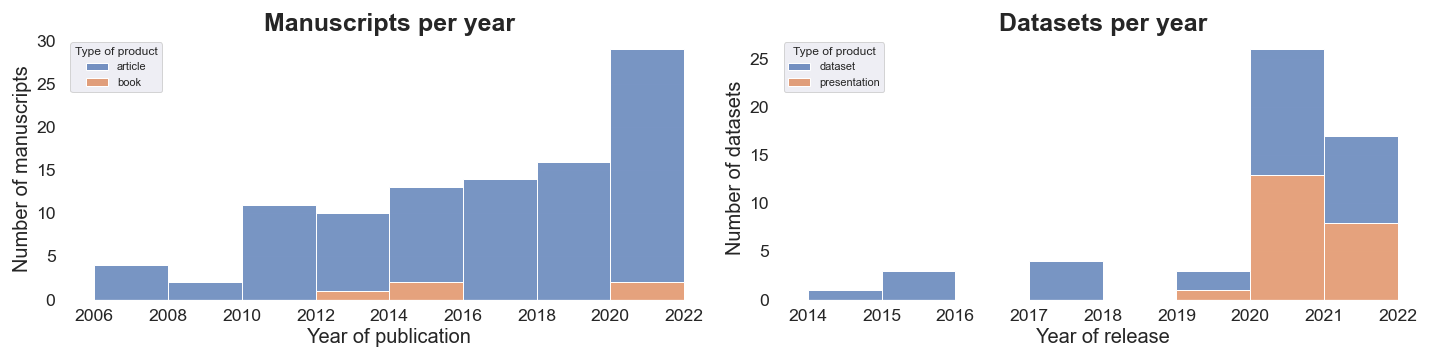
\includegraphics[width=\textwidth]{img/products_per_year.png}
\end{figure}

\begin{figure}[h]
\centering
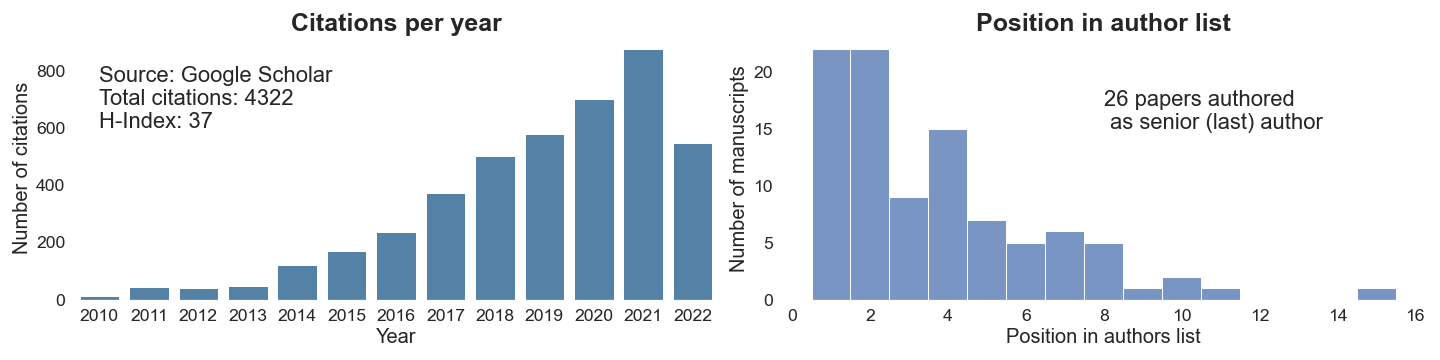
\includegraphics[width=\textwidth]{img/citations_authors.png} 
\end{figure}

\begin{figure}[h]
\centering
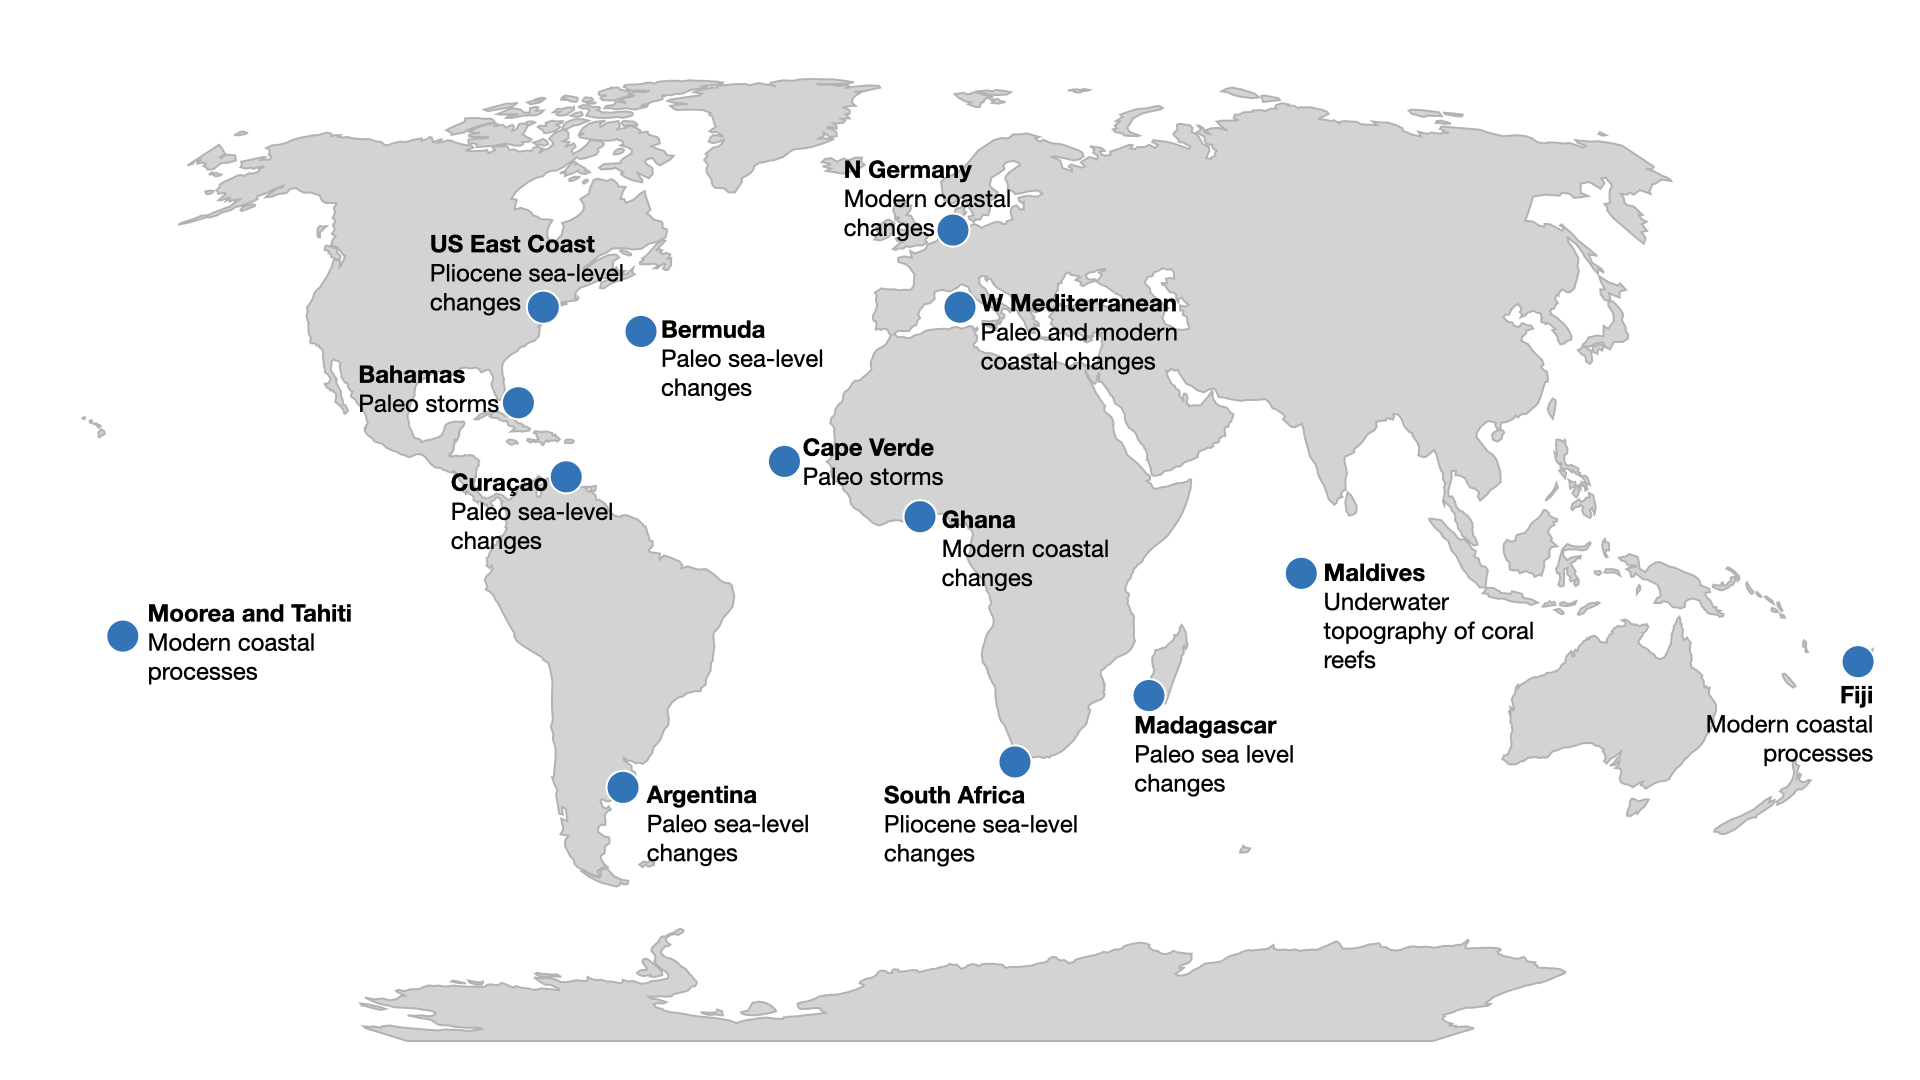
\includegraphics[width=0.95\textwidth]{img/field_data.png} 
\end{figure}

\clearpage

\pagestyle{empty}

\section[\faAreaChart]{List of publications}
Names of mentored postdocs, Ph.D. students or supervised students are \underline{underlined}

\nocite{*}
\section{\faBook \ \ \ Books and Book chapters}
I authored \textbf{4 book chapters} and \textbf{one textbook}
\printbibliography[type=book,heading=none]
\section{\faFileTextO \ \ \  Articles}
I authored \textbf{95 peer-reviewed articles}
\printbibliography[type=article,heading=none]
\section{\faFileTextO \ \ \  Open-access datasets}
Most products of my research are shared in open-access repositories
\printbibliography[type=dataset,heading=none]


%\nocite{*}
%\printbibliography

\end{document}